% $Header: /home/vedranm/bitbucket/beamer/solutions/generic-talks/generic-ornate-15min-45min.en.tex,v 90e850259b8b 2007/01/28 20:48:30 tantau $

\documentclass{beamer}

% This file is a solution template for:

% - Giving a talk on some subject.
% - The talk is between 15min and 45min long.
% - Style is ornate.



% Copyright 2004 by Till Tantau <tantau@users.sourceforge.net>.
%
% In principle, this file can be redistributed and/or modified under
% the terms of the GNU Public License, version 2.
%
% However, this file is supposed to be a template to be modified
% for your own needs. For this reason, if you use this file as a
% template and not specifically distribute it as part of a another
% package/program, I grant the extra permission to freely copy and
% modify this file as you see fit and even to delete this copyright
% notice.


\mode<presentation>
{
  \usetheme{Warsaw}
  % or ...

  \setbeamercovered{transparent}
  % or whatever (possibly just delete it)
}

      \newtheorem{proposition}[theorem]{Proposition}
      \theoremstyle{definition}
      \newtheorem{game}[theorem]{Game}
      \newtheorem{question}[theorem]{Question}

\usepackage[english]{babel}
% or whatever

\usepackage[latin1]{inputenc}
% or whatever

\usepackage{times}
\usepackage[T1]{fontenc}
% Or whatever. Note that the encoding and the font should match. If T1
% does not look nice, try deleting the line with the fontenc.


\usepackage{marvosym} % For \Smiley
\usepackage{verbatim} % for \verbatiminput

\usepackage{tikz}
\usetikzlibrary{matrix} % for diagrams

\title
{Game-theoretic strengthenings of Menger's property}

\subtitle
{29th Summer Conference on Topology and its Applications} % (optional)

\author%[Author, Another] % (optional, use only with lots of authors)
{Steven~Clontz~\\http://stevenclontz.com}%\inst{1} \and S.~Another\inst{2}}
% - Use the \inst{?} command only if the authors have different
%   affiliation.

\institute[Auburn University] % (optional, but mostly needed)
{
  %\inst{1}%
  Department of Mathematics and Statistics\\
  Auburn University}
  %\and
  %\inst{2}%
  %Department of Theoretical Philosophy\\
  %University of Elsewhere}
% - Use the \inst command only if there are several affiliations.
% - Keep it simple, no one is interested in your street address.

\date[14-07-23] % (optional)
{July 23, 2014}


% If you have a file called "university-logo-filename.xxx", where xxx
% is a graphic format that can be processed by latex or pdflatex,
% resp., then you can add a logo as follows:

 % \pgfdeclareimage[height=1cm]{university-logo}{auburn_logo.png}
 % \logo{\pgfuseimage{university-logo}}



% Delete this, if you do not want the table of contents to pop up at
% the beginning of each subsection:
%\AtBeginSubsection[]
%{
%  \begin{frame}<beamer>{Outline}
%    \tableofcontents[currentsection,currentsubsection]
%  \end{frame}
%}


% If you wish to uncover everything in a step-wise fashion, uncomment
% the following command:

%\beamerdefaultoverlayspecification{<+->}

% Strategy uparrow shortcuts
\newcommand{\win}{\uparrow}
\newcommand{\prewin}{\underset{\text{pre}}{\uparrow}}
\newcommand{\markwin}{\underset{\text{mark}}{\uparrow}}
\newcommand{\tactwin}{\underset{\text{tact}}{\uparrow}}
\newcommand{\kmarkwin}[1]{\underset{#1\text{-mark}}{\uparrow}}
\newcommand{\ktactwin}[1]{\underset{#1\text{-tact}}{\uparrow}}
\newcommand{\codewin}{\underset{\text{code}}{\uparrow}}
\newcommand{\limitwin}{\underset{\text{limit}}{\uparrow}}
\newcommand{\notprewin}{\underset{\text{pre}}{\not\uparrow}}
\newcommand{\notmarkwin}{\underset{\text{mark}}{\not\uparrow}}
\newcommand{\nottactwin}{\underset{\text{tact}}{\not\uparrow}}
\newcommand{\notkmarkwin}[1]{\underset{#1\text{-mark}}{\not\uparrow}}
\newcommand{\notktactwin}[1]{\underset{#1\text{-tact}}{\not\uparrow}}
\newcommand{\notcodewin}{\underset{\text{code}}{\not\uparrow}}
\newcommand{\notlimitwin}{\underset{\text{limit}}{\not\uparrow}}

\newcommand{\oneptcomp}[1]{#1^*}
\newcommand{\oneptlind}[1]{#1^\dagger}
% \newcommand{\sharp}[1]{#1^{\#}}

\newcommand{\congame}[2]{Con_{O,P}(#1,#2)}
\newcommand{\congamehard}[2]{Con_{O,P}^\star(#1,#2)}
\newcommand{\clusgame}[2]{Clus_{O,P}(#1,#2)}
\newcommand{\clusgamehard}[2]{Clus_{O,P}^\star(#1,#2)}

\newcommand{\lfkpgame}[1]{LF_{K,P}(#1)}
\newcommand{\lfklgame}[1]{LF_{K,L}(#1)}

\newcommand{\pfgame}[1]{PF_{F,C}(#1)}

\newcommand{\mengame}[1]{Cov_{C,F}(#1)}
\newcommand{\rothgame}[1]{Cov_{C,S}(#1)}
\newcommand{\altrothgame}[1]{Cov_{P,O}(#1)}

\newcommand{\fillgameS}[1]{Fill^{\cup,\subset}_{C,F}(#1)}
\newcommand{\fillgame}[1]{Fill^{\cup,\subseteq}_{C,F}(#1)}
\newcommand{\fillgameOne}[1]{Fill^{1,\subseteq}_{C,F}(#1)}
\newcommand{\fillgameInt}[1]{Fill^{\cap}_{C,F}(#1)}



\newcommand{\recallgame}[2]{Rec^{#1}_{F,S}(#2)}

\newcommand{\proxgame}[1]{Prox_{D,P}(#1)}
\newcommand{\aproxgame}[1]{aProx_{D,P}(#1)}

\newcommand{\SigmaProdR}[1]{\Sigma\mathbb{R}^{#1}}
\newcommand{\sigmaprodtwo}[1]{\Sigma2^{#1}}

\newcommand{\concat}{{^\frown}}
\newcommand{\rest}{\restriction}

\newcommand{\cl}[1]{\overline{#1}}

\newcommand{\pow}[1]{\mc{P}(#1)}

\newcommand{\<}{\langle}
\renewcommand{\>}{\rangle}

\newcommand{\mc}[1]{\mathcal{#1}}

\newcommand{\po}{\mathbb{P}}
\newcommand{\pok}{\po_\kappa}

\newcommand{\Lim}{\mathrm{Lim}}
\newcommand{\Suc}{\mathrm{Suc}}

\newcommand{\ds}{\displaystyle}

\newcommand{\st}[2]{st\left(#1,#2\right)}


\newcommand{\al}[1]{{#1}^*}
\newcommand{\alcomp}{\wr}

\newcommand{\rank}{\textrm{rank}}
\newcommand{\dom}{\textrm{dom}}

\renewcommand{\mod}{\,\textrm{mod}}

\newcommand{\zip}{\bowtie}
\newcommand{\ran}[1]{\text{range}(#1)}

\newcommand{\cf}[1]{\textrm{cf}(#1)}

\newcommand{\alcompS}[1]{S(#1,\omega,\omega)}


\newcommand{\scish}{almost-$\sigma$-(relatively compact)}

\usepackage{mathrsfs}
\newcommand{\pl}[1]{\mathscr{#1}}



\newcommand{\term}{\textit}


\newcommand{\bakergame}[1]{{Lim}_{A,B}(#1)}
\newcommand{\bmgame}[1]{{Empty}_{E,N}(#1)}




\begin{document}
% \renewcommand{\pause}{}
\newcommand{\vpause}{\pause\vspace{1em}}

\begin{frame}
  \titlepage
\end{frame}

% \begin{frame}{Table of Contents}
%   \tableofcontents
%   % You might wish to add the option [pausesections]
% \end{frame}


% \section{Introduction}

% \subsection{Abstract}

% \begin{frame}{Abstract}%{Subtitles are optional.}
%     \small
%     A certain topological game introduced by Hurewicz characterizes Menger's
%     covering property whenever the first player lacks a winning strategy. It
%     was later shown by Telgarsky (and later by Scheepers using a different
%     argument) that for metric spaces, the second player having a winning
%     strategy characterizes the stronger property of $\sigma$-compactness.

%     \vspace{1em}

%     We factor out Scheepers' proof to show
%     that for regular spaces, the second player having a winning $1$-Mark\"ov
%     strategy characterizes $\sigma$-compactness; also, for second-countable
%     spaces, the presence of a winning perfect information strategy for the
%     second player implies the existence of a winning $1$-Mark\"ov strategy for
%     that player. We also show the that for all $k$, the existence of a
%     winning $k$-Mark\"ov strategy for the second player implies the existence
%     of a winning $2$-Mark\"ov strategy, and give a space which permits
%     a winning $2$-Mark\"ov strategy but not a winning $1$-Mark\"ov strategy.
% \end{frame}

\section{Menger Spaces and the Menger Game}

\subsection{Definitions}

\begin{frame}{The Menger property}
  \begin{definition}
    A space $X$ is Menger if for every sequence $\<\mc U_0,\mc U_1,\dots\>$
    of open covers of $X$ there exists a sequence
    $\<\mc F_0,\mc F_1,\dots\>$ such that $\mc F_n\subseteq \mc U_n$,
    $|\mc F_n|<\omega$, and $\bigcup_{n<\omega}\mc F_n$ is a cover of $X$.
  \end{definition}

  \pause

  \begin{proposition}
    $X$ is $\sigma$-compact
      $\Rightarrow$
    $X$ is Menger
      $\Rightarrow$
    $X$ is Lindel\"of.
  \end{proposition}
\end{frame}

\begin{frame}{The Menger game}
  \begin{game}
    Let $\mengame{X}$ denote the \term{Menger game} with players
    $\pl C$, $\pl F$.
    In round $n$, $\pl C$ chooses an open cover $\mc C_n$,
    followed by $\pl F$
    choosing a finite subcollection $\mc F_n\subseteq \mc C_n$.

    $\pl F$ wins the game, that is, $\pl F \win \mengame{X}$ if
    $\bigcup_{n<\omega}\mc F_n$ is a cover for the space
    $X$, and $\pl C$ wins otherwise.
  \end{game}

  \pause

  \begin{theorem}
    $X$ is Menger if and only if $\pl C \not\win \mengame X$.
    (Hurewicz 1926, effectively)
  \end{theorem}
\end{frame}

\begin{frame}
  Menger suspected that the subsets of the real line with his property were
  exactly the $\sigma$-compact spaces; however:

  \pause

  \begin{theorem}
    There are $ZFC$ examples of non-$\sigma$-compact
    subsets of the real line which are Menger. (Fremlin, Miller 1988)
  \end{theorem}

  But metrizable non-$\sigma$-compact Menger spaces will be
  \term{undetermined} for the Menger game.

  \pause

  \begin{theorem}
    Let $X$ be metrizable. $\pl F\win\mengame X$ if and only if $X$ is
    $\sigma$-compact. (Telgarsky 1984, Scheepers 1995)
  \end{theorem}
\end{frame}

\subsection{Scheeper's Proof}

\begin{frame}
  Note that for Lindel\"of spaces, metrizability is characterized by regularity
  and secound countability.

  \vpause

  Sketch of Scheeper's proof:
  \begin{itemize}
    \item Using second-countability and the winning strategy for $\pl F$,
          construct certain subsets $K_s$ for $s \in \omega^{<\omega}$ such
          that $X = \bigcup_{s\in\omega^{<\omega}}K_s$.
    \item Using regularity, show that each $K_s$ is compact.
    \item The result follows since $|\omega^{<\omega}|=\omega$.
  \end{itemize}

  \vpause

  By considering winning \term{limited-information strategies}, we'll be able
  to factor out this proof a bit.
\end{frame}

\subsection{Limited information strategies}

\begin{frame}{Limited information strategies}
  \begin{definition}
    A \term{(perfect information) strategy} has knowledge of all the past
    moves of the opponent.
  \end{definition}

  \pause

  \begin{definition}
    A \term{$k$-tactical strategy} has knowledge of only the past $k$
    moves of the opponent.
  \end{definition}

  \pause

  \begin{definition}
    A \term{$k$-Mark\"ov strategy} has knowledge of only the past $k$
    moves of the opponent and the round number.
  \end{definition}
\end{frame}

\begin{frame}
  Obviously,
  \[
    \pl A \ktactwin{k} G
      \Rightarrow
    \pl A \kmarkwin{k} G
      \Rightarrow
    \pl A \underset{\text{(perfect)}}{\uparrow} G
  \]

  \vpause

  But tactical strategies aren't interesting for the Menger game.

  \begin{proposition}
    For any $k<\omega$,
    $\pl F\ktactwin{k}\mengame X$ if and only if $X$ is compact.
  \end{proposition}

  Effectively, $\pl F$ needs some sort of seed to prevent from being
  stuck in a loop: there's nothing stopping $\pl C$ from playing the
  same open cover during every round of the game.
\end{frame}

\section{$1$-Mark\"ov Strategies}

\subsection{Limited info and relative compactness}

\begin{frame}
  Comparitively, Mark\"ov strategies are very powerful.

  \begin{proposition}
    If $X$ is $\sigma$-compact, then $\pl F \kmarkwin{1}\mengame X$.
  \end{proposition}

  \begin{proof}
    Let $X=\bigcup_{n<\omega}K_n$. During round $n$, $\pl F$ picks a finite
    subcollection of
    the last open cover played by $\pl C$ (the only one $\pl F$ remembers)
    which covers $K_n$.
  \end{proof}
\end{frame}

\begin{frame}
  Without assuming regularity, we can't quite reverse the implication, but
  we can get close.

  \pause

  \begin{definition}
    A subset $Y$ of $X$ is \term{relatively compact} if for every open cover
    for $X$, there exists a finite subcollection which covers $Y$.
  \end{definition}

  \begin{proposition}
    If $X$ is $\sigma$-relatively-compact, then $\pl F \kmarkwin{1}\mengame X$.
  \end{proposition}

  \pause

  \begin{proposition}
    For regular spaces, $Y\subseteq X$ is relatively compact if and only if
    $\cl Y$ is compact. So $\sigma$-relatively-compact regular spaces are
    exactly the $\sigma$-compact regular spaces.
  \end{proposition}
\end{frame}

\begin{frame}

  \begin{theorem}
    $\pl F \kmarkwin{1}\mengame X$ if and only if $X$ is
    $\sigma$-relatively-compact.
  \end{theorem}

  \pause

  \begin{proof}
    Let $\sigma(\mc U, n)$ represent a $1$-Mark\"ov strategy.
    For every open cover $\mc U\in\mathfrak C$, $\sigma(\mc{U},n)$
    witnesses relative compactness for the set
      \[
        R_n
          =
        \bigcap_{\mc U\in\mathfrak C}\bigcup \sigma(\mc U,n)
      \]

    \pause

    If $X$ is not $\sigma$-relatively compact, fix $x \not\in R_n$ for any
    $n<\omega$. Then $\pl C$ can beat
    $\sigma$ by choosing $\mc{U}_n\in\mathfrak{C}$ during each round
    such that $x\not\in \bigcup\sigma(\mc{U}_n,n)$.
  \end{proof}
\end{frame}

\subsection{Limited info in second-countable spaces}

\begin{frame}
  So for regular spaces, a winning strategy for $\pl F$ in the Menger game
  isn't sufficient to characterize $\sigma$-compactness, but a winning
  $1$-Mark\"ov strategy does the trick.

  \vpause

  We can complete Telgarsky's/Scheeper's result by showing the following:

  \begin{theorem}
    For second countable spaces $X$, $\pl F \win \mengame X$ if and only if
    $\pl F \kmarkwin{1}\mengame X$.
  \end{theorem}
\end{frame}

\begin{frame}{Proof}
  Let $\sigma$ be a perfect information strategy.
  Since $X$ is a second-countable space, we may pretend that there are only
  countably many finite collections of open sets. Thus for
  $s\in\omega^{<\omega}$, we may define open covers $\mc U_{s\concat\<n\>}$
  such that for each open cover $\mc U$, there is some $n<\omega$ where
  \[
    \sigma(\mc U_{s\rest 1},\dots,\mc U_{s},\mc U)
      =
    \sigma(\mc U_{s\rest 1},\dots,\mc U_{s},\mc U_{s\concat\<n\>})
  \]

  \vpause

  Let $t:\omega\to\omega^{<\omega}$ be a bijection. During round $n$ and
  seeing only the latest open cover $\mc U$, $\pl F$ may play the finite
  subcollection
  \[
    \tau(\mc U,n) = \sigma(\mc U_{t(n)\rest 1},\dots,\mc U_{t(n)},\mc U)
  \]
\end{frame}

\begin{frame}{Proof (cont.)}
  Suppose there exists a counter-attack $\<\mc V_0,\mc V_1,\dots\>$ which
  defeats the $1$-Mark\"ov strategy $\tau$. Then there exists
  $f:\omega\to\omega$ such that, if $\mc V^n=\mc V_{t^{-1}(f\rest n)}$
  \[
    \begin{array}{rcl}
    x & \not\in & \bigcup \tau(\mc V^n,t^{-1}(f\rest n)) \\
    & = & \bigcup\sigma(\mc U_{f\rest 1},\dots,\mc U_{f\rest n},\mc V^n) \\
    & = & \bigcup\sigma(\mc U_{f\rest 1},\dots,\mc U_{f\rest n},\mc U_{f\rest (n+1)})
    \end{array}
  \]

  \vpause

  Thus $\<\mc U_{f\rest 1}, \mc U_{f\rest 2},\dots\>$ is a successful
  counter-attack by $\pl C$ against the perfect information strategy $\sigma$.
  \qed
\end{frame}

\section{$k$-Mark\"ov strategies for $k\geq 2$}

\subsection{$k$-Mark\"ov implies $2$-Mark\"ov}

\begin{frame}
  Unlike the Banach-Mazur game, we can immediately see that knowledge
  of more than two previous moves of $\pl F$'s opponent must be infinite
  to be of any use.

  \begin{theorem}
    If $\pl F \kmarkwin{k}\mengame X$, then $\pl F \kmarkwin2\mengame X$.
  \end{theorem}

  \begin{proof}
    \[
      \tau(\<\mc U,\mc V\>,n+1)
        =
      \bigcup_{m<k+2}
        \sigma(\<
          \underbrace{\mc U,\dots,\mc U}_{k+1-m},
          \underbrace{\mc V,\dots,\mc V}_{m+1}
        \>,(n+1)(k+2)+m)
    \]
  \end{proof}
\end{frame}

\subsection{$2$-Mark\"ov but not $1$-Mark\"ov}

\begin{frame}
  Knowledge of two previous moves versus one is an important distinction:
  in the former case, the player is able to react to change by the
  opponent.

  \pause

  \begin{definition}
    Let $\oneptlind\kappa = \kappa\cup\{\infty\}$ be the
    \term{one point Lindel\"of-ication} of discrete $\kappa$: neighborhoods
    of $\infty$ are exactly the co-countable sets containing it.
  \end{definition}

  \pause

  $\oneptlind\kappa$ is a simple space which is a regular and Lindel\"of, but
  not second-countable space or $\sigma$-compact. Thus
  $\pl F\notkmarkwin{1}\mengame{\oneptlind\kappa}$, but it's easy to see
  that $\pl F\win\mengame{\oneptlind\kappa}$. What about $2$-Mark\"ov
  strategies?
\end{frame}

\begin{frame}
  In 1991, Scheepers introduced the statement $\alcompS\kappa$ to study an
  infinite game involving the countable and finite subsets of $\kappa$.

  \pause

  \begin{game}
    Let $\fillgameS\kappa$ denote the \term{strict union filling game}
    with two players $\pl C$, $\pl F$. In round $0$, $\pl C$ chooses
    $C_0\in[\kappa]^{\leq\omega}$, followed by $\pl F$ choosing
    $F_0\in[\kappa]^{<\omega}$. In round $n+1$, $\pl C$ chooses
    $C_{n+1}\in[\kappa]^{\leq\omega}$ such that $C_{n+1}\supset C_n$, followed
    by $\pl F$ choosing $F_{n+1}\in[\kappa]^{<\omega}$.

    $\pl F$ wins the game if
    $\bigcup_{n<\omega} F_n\supseteq\bigcup_{n<\omega} C_n$; otherwise, $\pl C$
    wins.
  \end{game}
\end{frame}

\begin{frame}
  \begin{definition}
    For two functions $f,g$ we say $f$ is \term{almost compatible} with
    $g$ ($f\alcomp g$) if $|\{x\in\dom(f)\cap\dom(g):f(x)\not=g(x)\}|<\omega$.
  \end{definition}
  \pause
  \begin{definition}
    $\alcompS\kappa$ states that there exist functions
    $f_A:A\to\omega$ for each $A\in[\kappa]^{\leq\omega}$ such that
    $|f_A^{-1}(n)|<\omega$ for all $n<\omega$ and
    $f_A\alcomp f_B$ for all $A,B\in[\kappa]^\omega$.
  \end{definition}
  \pause
  \begin{theorem}
    $\alcompS{\omega_1}$; $Con(\alcompS{2^\omega}+\neg CH)$;
    $\neg\alcompS\kappa$ for $\kappa>2^\omega$.
  \end{theorem}
\end{frame}

\begin{frame}
  The round number is unnecessary in Scheeper's game, since $\pl C$ must
  choose strictly increasing sets.

  \begin{theorem}
    If $\alcompS\kappa$, then $\pl F\ktactwin2 \fillgameS\kappa$.
  \end{theorem}

  \pause

  As it turns out, a related game characterizes $\mengame{\oneptlind\kappa}$.

  \begin{definition}
    Let $\fillgameInt\kappa$ denote the \term{intersection filling game}
    analogous to $\fillgameS\kappa$, except that $\pl C$ has no restriction
    on the countable sets she choooses, but $\pl F$ need only ensure that
    $\bigcup_{n<\omega} F_n\supseteq \bigcap_{n<\omega} C_n$ to win
    the game.
  \end{definition}
\end{frame}

\begin{frame}
  \begin{theorem}
    $\pl F \kmarkwin{k} \mengame{\oneptlind\kappa}$ if and only if
    $\pl F \kmarkwin{k} \fillgameInt\kappa$.
  \end{theorem}

  \pause

  \begin{theorem}
    If $\alcompS\kappa$, then $\pl F\kmarkwin{2} \fillgameInt\kappa$.
  \end{theorem}

  \pause

  \begin{proof}
    Let $f_A:A\to\omega$ witness $\alcompS\kappa$. Then we define the
    winning $2$-Mark\"ov strategy $\sigma$ as follows:
      \[
        \sigma(\<A\>,0) = \{\alpha\in A: f_A(\alpha) = 0\}
      \]
      \[
        \sigma(\<A,B\>,n+1)
          =
        \{\alpha\in A\cap B
          :
        f_B(\alpha) \leq n+1
          \text{ or }
        f_A(\alpha)\not=f_B(\alpha)\}
      \]
  \end{proof}
\end{frame}

\begin{frame}
  \begin{corollary}
    $\pl F\kmarkwin{2}\mengame{\oneptlind\omega_1}$, but
    $\pl F\notkmarkwin1\mengame{\oneptlind\omega_1}$.
  \end{corollary}
  \begin{figure}
    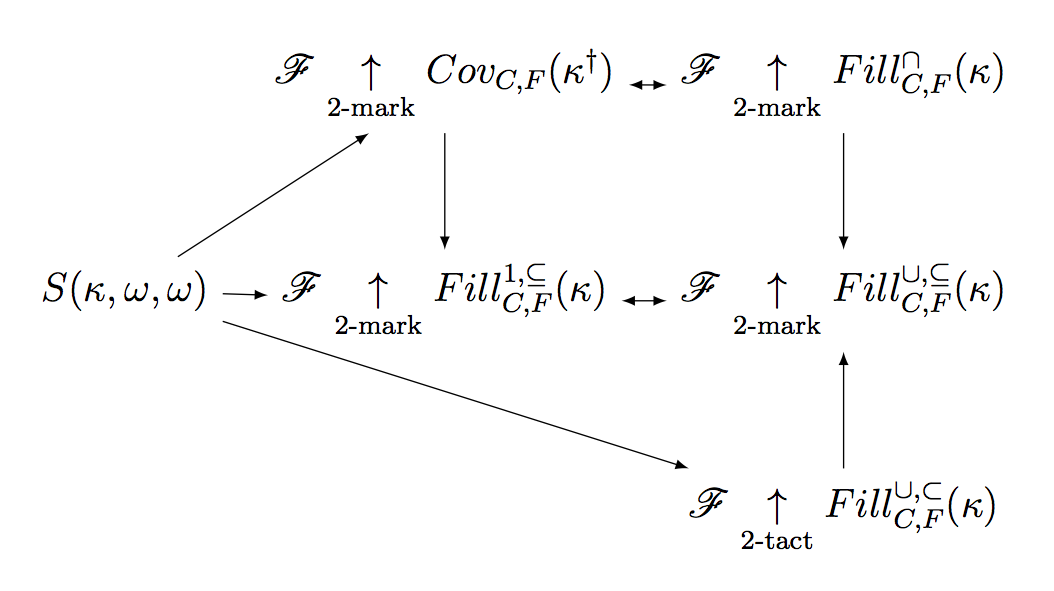
\includegraphics[height=1.7in]{mengerGameChart.png}
  \end{figure}
\end{frame}

\section{Quesitons}

\begin{frame}
  \begin{question}
    Does $\pl F\kmarkwin2\mengame{\oneptlind\kappa}$ imply $\alcompS\kappa$?
  \end{question}

  \pause

  \begin{question}
    Are $\pl F\win\mengame X$ and $\pl F\kmarkwin2\mengame X$ distinct?
  \end{question}

  An affirmative answer to the first question answers this since
  $\neg\alcompS\kappa$ for $\kappa>2^\omega$.
\end{frame}
\begin{frame}
  \begin{question}
    Where does $\pl F\kmarkwin2\mengame X$ fit in with other properties
    between $\sigma$-(relatively-)compact and Menger?
  \end{question}
  $\pl F\kmarkwin2\mengame X$ seems to characterize an
  ``almost-$\sigma$-(relative-)compactness''.

  \vpause

  Any sufficient property would imply $\pl F\win\mengame X$, and any
  (interesting) necessary property shouldn't be implied by
  $\pl F\win\mengame X$. Assuming $T_3$, properties which come to mind
  from the literature fit the latter: e.g. Alster (Aurichi, Tall 2013),
  and thus productively Lindel\"of (Alster 1988) and Hurewicz (Tall 2009).
\end{frame}

\section*{}

\begin{frame}
Questions? Thanks for listening!
\end{frame}


\end{document}


